%%%%%%%%%%%%%%%%%%%%%%%%%%%%%%%%%%%%%%%%%
% Stylish Article
% LaTeX Template
% Version 2.1 (1/10/15)
%
% This template has been downloaded from:
% http://www.LaTeXTemplates.com
%
% Original author:
% Mathias Legrand (legrand.mathias@gmail.com) 
% With extensive modifications by:
% Vel (vel@latextemplates.com)
%
% License:
% CC BY-NC-SA 3.0 (http://creativecommons.org/licenses/by-nc-sa/3.0/)
%1
%%%%%%%%%%%%%%%%%%%%%%%%%%%%%%%%%%%%%%%%%

%----------------------------------------------------------------------------------------
%	PACKAGES AND OTHER DOCUMENT CONFIGURATIONS
%----------------------------------------------------------------------------------------

\documentclass[fleqn,10pt]{SelfArx} % Document font size and equations flushed left

\usepackage[english]{babel} % Specify a different language here - english by default

\usepackage{marvosym, epigraph, subfig}

\usepackage[sortcites=false,style=authoryear-comp,bibencoding=utf8, natbib=true, firstinits=true, maxcitenames=2, maxbibnames = 99, uniquename=false, backend=bibtex, useprefix=true, backref=false,doi=false,isbn=false,url=false,dashed=true]{biblatex}
\setlength\bibhang{20pt}
\bibliography{ThomasReferenties.bib}
\AtEveryBibitem{%
	\clearfield{day}%
	\clearfield{month}%
	\clearfield{endday}%
	\clearfield{endmonth}%
}

%----------------------------------------------------------------------------------------
%	COLUMNS
%----------------------------------------------------------------------------------------

\setlength{\columnsep}{0.55cm} % Distance between the two columns of text
\setlength{\fboxrule}{0.75pt} % Width of the border around the abstract

%----------------------------------------------------------------------------------------
%	COLORS
%----------------------------------------------------------------------------------------

\definecolor{color1}{RGB}{0,0,90} % Color of the article title and sections
\definecolor{color2}{RGB}{0,20,20} % Color of the boxes behind the abstract and headings

%----------------------------------------------------------------------------------------
%	HYPERLINKS
%----------------------------------------------------------------------------------------

\usepackage{hyperref} % Required for hyperlinks
\hypersetup{hidelinks,colorlinks,breaklinks=true,urlcolor=color2,citecolor=color1,linkcolor=color1,bookmarksopen=false,pdftitle={What drives which region?},pdfauthor={Thomas de Graaff}}

%----------------------------------------------------------------------------------------
%	ARTICLE INFORMATION
%----------------------------------------------------------------------------------------

\JournalInfo{Research agenda, 2017--2021} % Journal information 
\Archive{Position paper} % Additional notes (e.g. copyright, DOI, review/research article)

\PaperTitle{Do regional economists answer the right questions?}
\SubPaperTitle{On the discrepancy between the questions regional economists solve and the questions policy makers actually ask}

\Authors{Thomas de Graaff\textsuperscript{1}*} % Authors
\affiliation{\textsuperscript{1}\textit{Department of Spatial Economics, Vrije Universiteit Amsterdam, Amsterdam, The Netherlands}} % Author affiliation
\affiliation{*\textbf{Corresponding author}: \Letter{} t.de.graaff@vu.n; \Mundus{} \href{thomasdegraaff.nl}{thomasdegraaff.nl}} % Corresponding author

\Keywords{Regional science --- spatial heterogeneity --- conditional robustness --- predicting --- data science}
\newcommand{\keywordname}{Keywords} 

%%----------------------------------------------------------------------------------------
%%	ABSTRACT
%%----------------------------------------------------------------------------------------

\Abstract{In this position paper I argue two things: namely, (\textit{i}) regional (or spatial) economists do not always answer the type of questions policy makers are concerned about, and consequently (\textit{ii}) they are very restrictive in the tool set they apply. First, policy makers---whether national, regional or local---are oftentimes concerned about holistic approaches and future predictions. Exemplary questions are ``What works best for my country/region/city'' and ``If we change this what will happen to the country/region/city as a whole?''. Regional economists---actually, most economists---usually isolate phenomena in order to, at best, explain the impact of a single determinant. Indeed, most regional economists feel very uncomfortable when asked to predict or give the best set of determinants for a certain phenomenon. This has its consequences for the tool set the regional economists applies. Usually a parametric regression type of framework is applied isolating the determinant under consideration and controlling as much as possible for unobservables and unobserved factors, ideally in a pseudo-experimental framework. A direct consequence of this approach is that emphasis is very much on explaining the impact of a determinant and not on predicting phenomena. For many applications that is definitely the right approach, however, as this paper forcefully aruges, it is very much as well a selective approach that does not do well to deliver on some of the questions policy makers ask regional economists.}

%----------------------------------------------------------------------------------------

\begin{document}

\flushbottom % Makes all text pages the same height
\maketitle % Print the title and abstract box
\tableofcontents % Print the contents section
\thispagestyle{empty} % Removes page numbering from the first page

%----------------------------------------------------------------------------------------

\section*{Introduction} % The \section*{} command stops section numbering

\addcontentsline{toc}{section}{Introduction} % Adds this section to the table of contents

\epigraph{The sexiest job in the next 10 years will be statisticians.}{Hal Varian, 2009}

The above quote from Hal Varian is in one aspect wrong; nowadays, we do not call them statisticians but data scientists instead. Nevertheless, in the last two decades companies such as Google, Ebay, Whatsapp, Facebook, Booking.com and Airbnb, have not only witnessed enormous growth but also changed the socio-economic landscape. Indeed, with the increasing abundance of (spatial) data and computer capacity, the ability to gather, process, and visualize data has become highly important and therefore highly in demand. And the models and tools, the data scientists within these companies use are very much \textit{data driven} with remarkable results 

Therefore it is striking 

\cite{breiman2001statistical}

%------------------------------------------------

\section{Background\label{Background}}

\begin{figure*}[ht]\centering 
	\subfloat[Model approach proces\label{modelapproach}]{%
		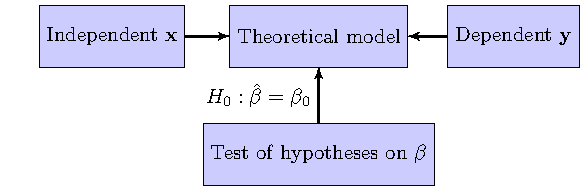
\includegraphics[width=0.48\textwidth]{./figures/modelapproach}
	}
	\hfill
	\subfloat[Data approach proces\label{dataapproach}]{%
		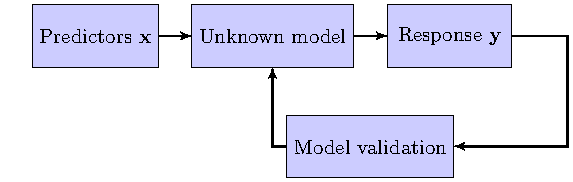
\includegraphics[width=0.48\textwidth]{./figures/dataapproach}
	}
	
	\caption{Two cultures of statistical/econometric modeling \citep[inspired by][]{breiman2001statistical}}
	\label{fig:twocultures}
\end{figure*}

Regions are conceptually different than cities, as they contain urban, suburban and rural areas simultaneously. Whilst smaller regions can still be seen as the total influence radius of metropolitan areas---such as measured by the concept of local labor markets and the NUTS-2 regions in Europe---, larger regions can typically contain a multiple of cities in combinations with their various hinterlands --such as the Dutch Randstad, the Belgian Flemish Diamond, and the German Ruhr areas. 

In recent years, the urban economics literature witnessed large growth; not only noticed by a wider acceptance in mainstream economics, but as well by larger scientific rigor and increased robustness of empirical findings. Remarkably, the empirical regional economics (or regional science in general for that matter) literature lagged behind, although many concepts and challenges in both disciplines are conceptually similar and are derived from similar theoretical backgrounds. 

Similar to urban economics\footnote{For this reason, in the UK in 2013 a new centre called \href{http://www.whatworksgrowth.org/}{``What Works Centre for Local Economic Growth''} led by Professor Henry Overman at the London School of Economics (LSE) has been established. This centre focuses mainly on the causal impact (impact evaluation) of investments at the city level.}, there is not yet a clear (consensus in) understanding in which policy instruments are actually (cost-)effective in promoting regional growth. 

To do so, I first review the previous literature in section \ref{Background}. This section focuses mainly on regional economics as it has a larger emphasis on \textit{causal} effects. To a lesser extent we deal with the (economic geography) literature. Based on this literature review Section \ref{gaps} deals with the research gaps that can be identified.


\begin{itemize}
	\item housing \& population; 
	\item amenities;
	\item connectivity \& accessibility
	\item networks;
	\item social \& humn capital
\end{itemize}

%------------------------------------------------

\section{Research gaps\label{gaps}}

%------------------------------------------------

\section{Research Agenda}


\subsection{Regional heterogeneity}

\citep{Thissen2016, Graaff2012, DeGraaff2012}

\subsection{Conditional robustness}

In regional science in general and in regional economics in specific, remarkably little attention has been given to reproducibility and robustness of results \citep[with some exceptions as, amongst some others, by][]{Rey:2014cl,arribas2015woow, Arribas2016}.

\subsection{Regional sorting models}

As in \citet{Bayer2004, Bayer2007a} and recently by \citet{Wang2016} and \citet{Bernasco2016}.


%----------------------------------------------------------------------------------------
%	REFERENCE LIST
%----------------------------------------------------------------------------------------

\addcontentsline{toc}{section}{References} % Adds this section to the table of contents
\printbibliography

%----------------------------------------------------------------------------------------

\end{document}